%% We use `subfiles' package
\documentclass[preamble.tex]{subfiles}
\begin{document}

\clearpage

\chapter{Loop representation: The Loop Language}

\LiveFusion at the top level is a library of high level array combinators. Most of these conceptually represent a loop. Indeed, the user of the library can reason about the individual combinators as loops and consider the result of each to be an array.

However, when running the user's program, we are aiming to perform the required operations in as few loops as possible\footnote{This may increase register pressure. However, unless register spilling poses a problem in the future we favour the decreased memory traffic which is attained by array fusion.}. \todo{We have discussed the conditions for fusible combinators in Section ... In general, however...} Subject to certain restrictions, two combinators in \LiveFusion are fusible when the output array \*produced* by one combinator is \*consumed* as input by another combinator one element at a time from beginning to end.

In the \LiveFusion AST discussed in the previous chapter, this relationship is usually seen between a child node (the producer) and its parent node (the consumer). This is not true for \*random access* combinators like @backpermute@ which we discuss separately\todo{in Section }.

\todo{How do we know whether two combinators can be fused?}Intuitively, two combinators can be fused whenever one could write a loop by hand which would give the same final result for the same input as the two separate loops would.
%We need a way to programmatically determine whether a given pair of combinators can be replace with a semantically equivalent loop.

%The focus of this chapter is to establish the requirements for fusible combinators and define a loop representation to which such fusible combinators can be mapped.
The focus of this chapter is to establish a common loop representation to which fusible combinators can be mapped.

In the following sections we will look more closely at what a loop really is and then present the core of our fusion optimisation.


\section{Anatomy of a loop}
\label{sec:anatomy}

Despite the purely functional, combinatorial interface to the library, looking at a loop in a procedural way is the approach I have opted for in the middle layer of the system. It is represented by the \Loop language\iloop{}.

The loops \LiveFusion generates can be viewed as similar to those one might write in an Assembly language. It uses labelled basic blocks and has explicit control flow using @goto@ statements\footnote{The formal grammar of the \Loop language is introduced later in the chapter. It is presented in Figure \ref{fig:Loop-grammar} on \pageref{fig:Loop-grammar}}.

However, as we will see later, they are often even more structured than loops in \C and other mainstream procedural languages. As such I urge the reader to think of them as being high-level and treat the explicit control flow as implementation details.

%The downside, however, is that our loop relies on \|goto|-like statements whose use is almost always considered bad practice in modern software engineering.

Without further delaying the discussion of the matter we will now look are the structure of a typical @for@ loop in a language like \C in an attempt to shape our own loop structure.


\subsection{Structure of a \code{for} loop}

Consider the following fragment of a \C program that creates a new array @ys@, by applying some function @f@ to those elements of array @xs@ that satisfy some predicate function @p@ (in \Haskell this could be expressed as @ys = (filter p . map f) xs)@):

\begin{ccode}[numbers=left]
int *ys = malloc(len * sizeof(int)); // result array
int i = 0;                          // output index
for(int i = 0; i < len; i++) {
    if(p(xs[i])) {
        ys[j] = f (xs[i]);
        j++;
    }
}
ys = realloc(ys, o * sizeof(int));
\end{ccode}

A @for@ loop in \C has four sections:

\begin{enumerate}
\halfspacing
\item \*initialisation* section (@i = 0@),
\item \*guard* section (@i < len@),
\item the main \*body* (@if(){ $...$ }@), and finally
\item the \*update* section (@i++@).
\end{enumerate}

Compared to free-formed @while@ loops which only have a @guard@ and a @body@, the @for@ loops are already much more structured.

However, as we will now show, further structural elements could be introduced which will ultimately assist us when composing loops from array combinators.


\subsubsection{Initialisation}

The very first observation to make is that both the result array @ys@ and the output index @j@ were declared and initialised outside the @for@ loop.

In pursuit of a more structured and composable approach to looping the \Loop language all statements executed \*once* before the loop begins are placed in the \[init] basic block of the loop.nn

The initialisation code corresponds to the following in the \Loop language:

\begin{loopcode}
init:
  let len = arrayLength xs
  let ys = newArray len
  let i = 0
  let j = 0
  goto guard
\end{loopcode}


\subsubsection{Guard}

The @guard@ of a @for@ loop corresponds to a \[guard] block of in the \Loop language. It can contain arbitrary statements but usually contains at least one @unless@ statement:

\begin{loopcode}
guard:
  unless i < len | done
  goto body
\end{loopcode}

The @guard@ \*statement* transfers the control to a different block if the condition is \*false* (to \[done] in this case).


\subsubsection{Update}

The @update@ equivalent of a @for@ loop in the \Loop language is the basic block called \[bottom]:

\begin{loopcode}
bottom:
  i := i + 1
  goto guard
\end{loopcode}

The block so called because it is executed \*unconditionally* at the end of each iteration.

As seen in the code above \Loop language supports destructive updates through using @assignment@ (@:=@).


\subsubsection{Finalisation}

The @filter@ results in a shorter array in the general case. Hence, after the @for@ loop finishes, the resulting array is \texttt{realloc}'ated to free the unused memory (in practice the array is unlikely to be copied).

This is one of the use cases for what is called a \[done] block of the loop:\todo{As we will see later it is not only useful for trimming and returning the final array but also for scheduling other loops such as in @append@ combinator.}.

\begin{loopcode}
done:
  let result = sliceArray ys j   -- resize to length j
  return result
\end{loopcode}

As seen from the code, every loop has a result which it returns explicitly.


\subsection{``Dissecting the bodies'' of loops}

We will now attempt to categorise the types of operations that all belong to the bodies of conventional @for@ and @while@ loops.

\subsubsection{Reading and writing arrays}

Line 5 of the @for@ presented above (@ys[j] = f (xs[i]);@) is actually doing three things:
\begin{enumerate}
\halfspacing
\item \*reading* an element from array @xs@,
\item \*producing* a new element by applying @f@ to it, and
\item \*writing* the new element into array @ys@.
\end{enumerate}

Consider, however, that we are trying to devise a loop representation for an application of fusion. When several combinators are fused into a single loop and produce no intermediate arrays, such reading and writing only happens at the beginning and at the end of a combinator pipeline.

Hence we want to separate the notion of \*producing* a new element from the fact that it came from an array, a list or just another computation. Likewise, we do not need to be concerned with how the new element is going to be consumed. It may or may not be written into a new array. It may or may not be used by a consuming combinator. However, it should not up to an individual combinator to decide.

In fact, an element may not even be produced as we discuss next.


\subsubsection{Skip producing an element}

Combinators like @filter@ may not produce a new element in every iteration. This was the case with the example above where only elements satisfying predicate @p@ were used. The \*guard* of the @if@ was serving as a predicate check which its body was the code that produced the element.

The \Loop language attempts to be more precise about where the element is produced. The code is split across two blocks: \[body] and \[yield]:

\begin{loopcode}
body:
  let x = readArray xs i
  unless (p x) | bottom  -- end iteration if the predicate is not satified
  let y = f x
  goto yield

yield:
  writeArray ys j y
  j := j + 1
  goto bottom
\end{loopcode}

The \[body] block deals with all the code that is concerned with producing an element, however an element is known to have been produced only if it the control reaches the \[yield] block.

This allows us to make assumptions about the behaviour of a loop without knowing what the loop is doing internally. As we will see later, the code that introduces @writeArray@ statements into the loop is oblivious to how the element has been produced. It knows that an element has definitely been produced if the control enters the \[yield] block.


\subsection{The complete example}

We have now constructed a complete loop in the internal \Loop language which corresponds to the \C code at the beginning of the section. The \C code in turn corresponds to \Haskell program @ys = (map f . filter p) xs@.

Both the original program and the resulting loop are given in Figure~\ref{fig:MapFilter}.


\begin{figure}

\begin{subfigure}{.5\textwidth}
\begin{loopcode}
init:
  let len = arrayLength xs
  let ys = newArray len
  let i = 0
  let j = 0
  goto guard

guard:
  unless i < len | done
  goto body

body:
  let x = readArray xs i
  unless (p x) | bottom
  let y = f x
  goto yield

yield:
  writeArray ys j y
  j := j + 1
  goto bottom

bottom:
  i := i + 1
  goto guard

done:
  let result = sliceArray ys j
  return result
\end{loopcode}
\end{subfigure}%
%
\begin{subfigure}{.5\textwidth}
\begin{ccode}
int *ys = malloc(len * sizeof(int));
int i = 0;
for(int i = 0; i < len; i++) {
    if(p(xs[i])) {
        ys[j] = f (xs[i]);
        j++;
    }
}
ys = realloc(ys, o * sizeof(int));
\end{ccode}
\end{subfigure}

\caption{Computation \code{ys = (map f . filter p) xs} in \C (right) and internal \Loop language (left).}
\label{fig:MapFilter}
\end{figure}


\section{The \Loop language more formally}
\label{sec:The-Loop-language}
\iloop{}

In summary we have used the following features of the \Loop language in the previous example:
\begin{enumerate}
\halfspacing
\item New variable binding (@i = 0@)
\item Variable assignment (@i := i + 1@)
\item Explicit control transfer (@goto body@)
\item Conditional control transfer (@guard i < len | done@)
\item Returning values from loop (@return ys'@)
\item A number of built-in array primitives: (@newArray@, @readArray@, @writeArray@, @arrayLength@ and @sliceArray@).
\end{enumerate}

All of the above are \*statements*, which are grouped into labelled \*basic blocks*\iblock.

The grammar of the \Loop language is presented formally in Figure~\ref{fig:Loop-grammar}. The syntax seen in the examples throughout this thesis is the same as used by the pretty printer for the language and it faithfully reproduces the internal representation of \Loop programs.

\begin{cfigure}{\label{fig:Loop-grammar}Grammar of \Loop language.}
\subfile{loop-grammar}
\end{cfigure}
\todo{Put the footnotetext on the same page where the grammar ends up}\footnotetext{For improved readability the unique integers are replaced with meaningful names in the code listings.}

If the grammar is studied more carefully one would note two each basic block may have multiple associated labels. As we will see in the next section this is a vital feature of the language which allows for easy fusion of loops.

We also note that each label and variable in the language is postfixed with a unique value which has so far been omitted from the listings.


\section{Loop generation}

In the previous section we have seen the first example of the \Loop EDSL which computed at @filter@ of an array followed by a @map@. We have also identified five main \*sections* of a loop, represented by \*basic blocks* in the \Loop language: \[init], \[guard], \[body], \[yield], \[bottom] and \[done].

We shall revisit the example from the previous section and introduce the process by which a \Loop is generated.

This time we extend the example with specific functions passed to @map@ and @filter@ combinators. The function @toPercentages@ shown on Figure~\ref{fig:toPercentages} (left) converts an array fractions to their percentage equivalents, filtering out those below $0.01$ (or $1\%$).

\begin{figure}
\begin{subfigure}{.65\textwidth}
\begin{hscode}
toPercentages :: Array Double -> Array Double
toPercentages fractions
  = let significant = filter (>=. 0.01) fractions
        percents    = map (* 100) significant
    in  percents
\end{hscode}
\end{subfigure}%
%
%\begin{subfigure}{.3\textwidth}
%  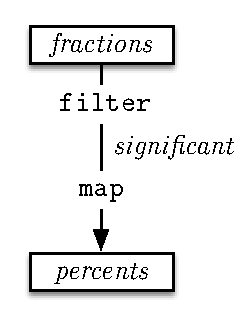
\includegraphics[height=12em]{img/toPercentages-flow}
%\end{subfigure}
%
\begin{subfigure}{.35\textwidth}
  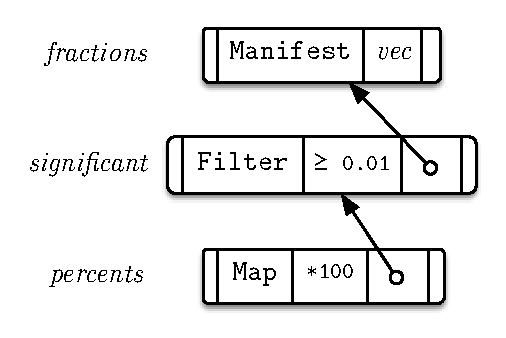
\includegraphics[height=10em]{img/toPercentages-ast}
\end{subfigure}
\caption{\code{toPercentages} function (left) and its \LiveFusion AST (right).}
\label{fig:toPercentages}
\end{figure}


\subsection{Start with an AST}

The @toPercentages@ function internally uses a pipeline of to combinators: the output array of @filter@ (@significant@) becomes the input array of @map@. Remembering that @Array Double@ is the type synonym for @AST (Vector Double)@, each combinator constructs a node in an AST representing a \*delayed array computation*.

It is impossible possible to know statically whether the input @fraction@ array is computed by a long pipeline of combinators or is a @Manifest@ array stored in memory. Likewise, it is not known before the runtime if the resulting @percents@ array is consumed by another combinator and the pipeline of delayed operation will continue to grow after @toPercentages@ function returns.

For the purposes of illustration we will assume that the @toPercentagee@ function is called with a @Manifest@ array as argument and the result is immediately \*forced* to be computed (e.g. to be printed out or to be consumed in a random access fashion).

In this case the AST shown on Figure~\ref{fig:toPercentages} (right) is constructed and \*forced* to a @Manifest@ array at the runtime of the program:

\begin{hscode}[mathescape]
-- AST that may be generated for a call to toPercentages
ast :: AST (Vector Double)
ast = force $\dol$ Map (* 100) $\dol$ Filter (>=. 0.01) $\dol$ Manifest vec

-- LiveFusion library functions
force :: Elt a => AST (Vector a) -> AST (Vector a)
force = Manifest . evalArrayAST

evalArrayAST :: Elt a => AST (Vector a) -> Vector a
evalArrayAST = $...\ compile\ AST\ and\ compute\ result ...$
\end{hscode}

The three fusible combinators (@Manifest@, @Filter@ and @Map@) are followed by the call to an evaluator, which processes them individually as shown next.
% After sharing recovery each AST node (or rather ASG node) is assigned a unique value


\subsection{Generate loops for individual combinatos}

In order to generate the \Loop code for an AST of combinators, the evaluator first processes them individually. For each combinator it populates the parts of the loop that were identified in Section~\ref{sec:anatomy}. It does so by inserting new statements into the corresponding basic blocks thus instantiating the loop template.

\subfile{lst-toPercentages-loops}

The left of Figure~\ref{fig:toPercentages-loops} presents
Recalling

It is now time to remember the \|Manifest| combinator of LiveFusion language that we used to bring a physical array in memory and create a LiveFusion language term out of it. As it turns out, \thesis{all the reading of physical arrays is performed by the code generated by the \|Manifest| combinator}. What this means is that, while the reading is still performed in the \|body| code block of of the loop, the code for it is only generated once at the beginning of each combinator pipeline.

Applied to the function from our $aboveThreshold$ example, this tells us that since we don't know which combinator produced the $xs$ array, the loop code generated for the $aboveThreshold$ function will *not* inlcude the specifics of where the individual elements of $xs$ came from.

\begin{loopcode}
  -- Loop: adjusted = \|map| f xs
  init_adj:
    goto guard_adj

  guard_adj:
    goto body_adj

  body_adj:
    elt_adj = f elt_xs
    goto yield_adj

  yield_adj:
    goto bottom_adj

  bottom_adj:
    goto guard_adj

  done_adj:


  -- Loop: above = \|filter| (>100) adjusted
  init_abv:
    o_abv = 0
    goto guard_abv

  guard_abv:
    goto body_abv

  body_abv:
    elt_abv = elt_adj
    guard (elt_abv > 100) bottom_abv
    goto yield_abv

  yield_abv:
    o_abv := o_abv + 1
    goto bottom_abv

  bottom_abv:
    goto guard_abv
\end{loopcode}

One will immediately notice the absence of loop counters $i$, array read/writes or allocations. Instead we only see some references to undeclared variables $elt_xs$, $elt_adj$, $elt_abv$. These represent the values of elements of $xs$, $adjusted$ and $above$ arrays at each iteration\footnote{In our implementation all variables, block labels and AST/ASG nodes are given a unique label, an integer. For readability we replaced those with meaningful subscripts.}

It is clear that these two loops are incomplete and cannot be run by themselves. Now suppose that the function $aboveThreshold$ is actually applied to some manifest array $xs$ (where $xs$ is a Vector in current implementation) and that the result of this application is forced to a manifest array, for example:
% Perhaps the manifest array should be stored with the node in an IORef/M
\begin{hscode}
let accepted = aboveThreshold abs (Manifest xs)
in  ...random access $accepted$...
\end{hscode}

What happens is that two new loops are generated: one for \|Manifest| $xs$ and one for the physical array creation:

\begin{loopcode}
  -- Loop: \|Manifest| xs
  init_xs:
    len_xs = arrayLength xs
    i_xs = 0
    goto guard_xs

  guard_xs:
    guard (i_xs < len_xs) done_xs
    goto body_xs

  body_xs:
    elt_xs = readArray xs i_xs
    goto yield_xs

  yield_xs:
    goto bottom_xs

  bottom_xs:
    i_xs := i_xs
    goto guard_xs

  done_xs:


  -- Loop: forcing aboveThreshold f xs
  init_force:
    result = newArray len_xs
    goto guard_force

  guard_force:
    goto body_force

  body_force:
    goto yield_force

  yield_force:
    writeArray result o_abv elt_abv
    goto bottom_force

  bottom_force:
    goto guard_force

  done_force:
    result := sliceArray result o
\end{loopcode}

The \|Manifest| loop is the only one of the four ``loops'' presented so far that actually resembles a runnable loop. Out of the four it is the only one that introduces a source array counter $i_{xs}$ in the \|init| block which it compares against the length of $xs$ in the \|guard|. It also increments it in the \|bottom| block.

All in all the \|init|, \|guard| and \|bottom| blocks of the \|Manifest| $xs$ loop resemble very closely the \|initialisation|, \|guard| and \|update| section of the \|for| loops we presented earlier in our C version of the function. We will revisit this comparison very soon.

We have essentially given the complete Loop representation for \|Manifest|, \|map| and \|filter| combinators together with the code that actually deals with writing out physical arrays. However, it all came in separate loops none of which was very useful by itself. We will now show how these loops can be turned into a runnable loop.

\subsubsubsection{Merging loops}

In the previous section we have established how each of the combinators of the $aboveThreshold$ function contribute to each loop. Each of those loops has \|init|, \|guard|, \|body|, \|yield|, \|bottom| and \|done| code blocks which are connected by \|goto|s. We can now simpy merge the respective sections of all loops to give a loop in Figure . The statements of \|Manifest| array itteration preceed those of the \|map|, which in turn preceed those of the \|filter|. The statements of physical array creation come last.

\begin{loopcode2}[%
    caption={Final loop for a call of aboveThreshold Function.},
    label=lst:aboveThreshold-final-loop,
    literate=
      {_xs}{{\sub{xs}}}2
      {_abv}{{\sub{abv}}}3
      {_adj}{{\sub{abv}}}3
]
  -- Loop: force $\char36$ filter (> 100) $\char36$ map f $\char36$ Manifest xs
  init:
    len_xs = arrayLength xs          -- From \|Manifest|
    i_xs = 0                         -- From \|Manifest|
    o_abv = 0                        -- From \|filter|
    result = newArray len_xs         -- From forcing result
    goto guard

  guard:
    guard (i_xs < len_xs) done       -- From \|Manifest|
    goto body

  body:
    elt_xs = readArray xs i_xs       -- From \|Manifest|
    elt_adj = f elt_xs               -- From \|map|
    elt_abv = elt_adj                -- From \|filter|     
    guard (elt_abv > 100) bottom     -- From \|filter|
    goto yield

  yield:
    o_abv := o_abv + 1               -- From \|filter|
    writeArray result o_abv elt_abv  -- From forcing the result
    goto bottom

  bottom:
    i_xs := i_xs                     -- From \|Manifest|
    goto guard

  done:
    result := sliceArray result o   -- From forcing result
\end{loopcode2}

Talk about loop merging........

An important difference however, is that while in the C version there were two separate loops with separate counters ...



\section{More on \|goto|'s}

While the use of \|goto|'s is considered bad practice in modern software engineering we note several reasons for using them in our intermediate language:

\begin{itemize}
  \item It is completely hidden from the library user. Given a well behaving Loop code generator the produced code will always be valid if the user program is valid. This is akin to using \|unsafePerformIO| and similar combinators within the guts of the library for performance reasons. They can lead to bad code but with careful use give very noticeable advantages to purely functional programs.

  \item The library was designed with pluggable backend in mind. It was assumed that assembly-like Loop language would be easier to connect with any backend. Specifically for Haskell backend, \|goto| statements are translated to tail-recursive function calls.

  \item The \|goto|-based design seemed to be the most flexible and the easiest to implement. None-the-less, the Loop language may be extended to support a safer and more advanced implementation where individual *blocks* become functions.
\end{itemize}








\section{Block names}

+ Many of the combinators use a similar set of variables, e.g. both Map and Scan produce a value at each iteration which they assign to an intermediate variable in the body of the loop, say elt
+ Thus if there are two maps one after the other, we need to distinguish between the two
+ We give earch such variable a unique identifier which coincides with the identifier of the combinator in the graph (see section), e.g. $elt_3$ is always an intermediate element produced by combinator 3 in each iteration (provided the combinator is a producer)
+ Other examples include $len_3$, $len_1$, $i_1$, $o_5$, $acc_4$
+ Not only this removes any potential name clashes (since ids are unique), but also allows us to refer to any variable in the loop just knowing what function it's performing as well as the combinator id.
+ When is it useful? Can we have a DS passing those variables without stupid conventions?
+ The problem is that the names are generated by convention, so in case of any error, the program would either fail to compile at runtime or produce incorrect results
+ The easiest way 
+ Like global variables
+ Spooky action at a distance
+ Untracked interaction between different parts of loop
+ In many cases a flaw of software design, often discouraged and even semantically prohibited in functional languages like haskell and ml.



\section{Communication by Convention}

We have discussed that our loop clauses are being populated by combinators that do not know how many other combinators are in the pipeline or what these combinators are. And yet, once all of the combinators have filled in their parts, we end up with just one loop in which those combinators operate on the shared state. We will now discuss the approach by which those combinators cooperate with each other inside a single loop and how the state produced by one combinator is passed on to the combinators in the subsequent parts of the pipeline.

Let's look a simple example of what shared state a pipleline of two combinators @map g $ map f $ xs@ is.


\subsection{Intermediate values}
\label{sec:Loop:Elts}

As usual we decompose each combinator into a set of loop clauses. We have done this for the \|map| combinator in the previous section. However, the added complication is that there are two \|map|s, both of which expect an input value in $elt_i$ and and produce an output value in $elt_o$ at each iteration. This results in variable name clashes. We could give them unique names $elt_{i_1}$, $elt_{o_1}$, $elt_{i_2}$ and $elt_{o_2}$ based on the number of the combinator in the pipeline. We also notice that the output $elt_{o_1}$ of \|map f| is fed as input $elt_{i_2}$ to \|map g|. A simple solution is to introduce an equation $elt_{i_2} = elt_{o_1}$ for each combinator. This is the first example of interaction between combinators through shared state.
 $elt_{i_2} = elt_{i_1}$ might not be terribly exciting to read about

In the above example, we have established that for combinators that consume one element in each iteration, such as \|map|, \|fold| or \|filter|, that element would be stored in variable $elt_{o_n}$ where *n* is the the unique number of the previous combinator in the pipleline. The prefix $elt_o$ is its generic form and designates the intermediate output value in an iteration. This is the first *convention* that we use in our *Loop* language to tie together the code generated by different combinators.

The two combinators |map g . map f| give us code similar to the following:

\begin{loopcode}
body:
  elt_{i_1} = elt_{o_0}          -- input  of `map f'
  elt_{o_1} = f elt_{i_1}  -- output of `map f'
  elt_{i_2} = elt_{o_2}          -- input  of `map g'
  elt_{o_2} = g elt_{i_1}  -- output of `map g'
\end{loopcode}

\subsection{Loop counters}

Another important *convention* that the Loop language uses in every loop it generates are the loop counter variables.
%% As we will see later the naming convention is not only used to tie the code together but also gives rise to an optimisation and provides a solution to duplicated loop counters identified in Section (TODO ref).

The variables holding the *elements* of intermediate arrays we saw in the previous section are used in each cycle of the loop but do not represent the state that is carried over to the next iteration. The *loop counters* on the other hand are *mutable* variables that are destructively updated on each iteration and for part of the loop's state.

The most obvious place to introduce the counter variable is the \|Manifest| combinator which lifts a physical array into the *LiveFusion* EDSL. It is required to produce an element in each iteration of the loop by indexing the physical array that it wraps. Therefore, the index is not simply the loop's overall state, but the state of the \|Manifest| combinator.

To introduce this loop counter state we need to do the following:

In the \|init|ialisation clause of the loop:
+ declare the counter variable
+ assign it the initial value of 0
+ declare length variable
+ assign it the length of the array

In the \|guard|:
+ check if we have reached the end of the array
+ exit the the loop if we have

In the \|bottom| clause of loop which deals with updating the state:
+ increment the variable using destructive update

Following the above steps introduces the loop counter into the loop. The remaining implementation of \|Manifest| combinator resides in the main \|body| of the loop:
+ declare an intermediate value $elt_o$ and read the physical array at the appropriate index into it

The complete loop definition resulting from lifting a physical array into LiveFusion EDSL using \|Manifest| combinator is shown in Figure (TODO ref).

\begin{loopcode}
init:
  len_0 = length xs
  i_0   = 0

guard:
  pred_0 = i_0 < len_0
  guard pred_0 done        -- goto done block if the predicate is false

body:
  elt_{o_0} = read xs i_0

bottom:
  i_0 = i_0 + 1

done:

\end{loopcode}


\subsection{Merging Loops}

Coming back to our example of \inlc{map g \$ map f \$ xs} we now have both the code lifting \|xs| into the loop computation as well as the code for the \|map|s. Since theses are all part of the same loop, we can merge the statements from the same loop clauses into one loop. In this case the \|map| combinators really only had statements in the \|body| so this is the one clause which actually demonstates the loop merging\footnote{Technically, there are three loops which are generated and merged together: one for the manifest array, one for |map f| and one for |map g|. We initially omitted the merging process for |map g \compose map f| expression to avoid introducing too many concepts at a time.}:

\begin{loopcode}
init:
  -- Manifest xs
  len_0 = length xs
  i_0   = 0

guard:
  -- Manifest xs
  pred_0 = i_0 < len_0
  guard pred_0 done        -- goto done block if the predicate is false

body:
  -- Manifest xs
  elt_{o_0} = read xs i_0
  -- Map f
  elt_{i_1} = elt_{o_0}          -- input  of `map f'
  elt_{o_1} = f elt_{i_1}  -- output of `map f'
  -- Map g
  elt_{i_2} = elt_{o_2}          -- input  of `map g'
  elt_{o_2} = g elt_{i_1}  -- output of `map g'

bottom:
  -- Manifest xs
  i_0 = i_0 + 1

done:

\end{loopcode}




\subsection{Writing out the result}

So far we have demonstrated how we can turn a number of consecutive combinators into a single loop. Even though conceptually each of those is producing a new array, we have avoided writing it out to a physical array. However, all we are doing now is just burning CPU cycles producing some new values at each loop iteration and immediately forgetting about them. We need a way to return results from the loop. Thus for the last combinator in the loop we need to introduce some extra code which would:
+ **Allocate** a mutable array of appropriate size to write the result into\\
  This is done only once in \|init| block.
+ **Write** into it at the appropriate index whenever the next element is produced\\
  We introduce a new loop block for that called \|write|. By default it is entered after the \|body| loop is finished. The reason for having a separate block for that will become apparent when we dicsuss filters (Section \ref{sec:Loop:Filt})
+ **Resize and freeze** the mutable array to an immutable one when the array is complete\\
  Again, only done once in the \|done| block

We introduce one other important convention our combinators follow. We saw in Section \ref{sec:Loop:Elts} on Intermediate Values that each combinator sees its input element in variable $elt_{i_n}$, where $n$ is a unique number of the combinator. The combinator is not concerned with how this variable came to be. The Loop language framework takes care of bringing this variable into the scope of the combinator.

Following this approach, if the combinator 2 consumes elements produced by combinator 1 at the same index, then the Loop language automatically updates the index for combinator 2 (i.e. $i_2$ = $i_1$). This way, writing out the result of combinator 2 is as easy as generating a statement `writeArray $arr_2$ $i_2$ $elt_{o_2}$'.

\begin{loopcode}
init:
  -- Manifest xs
  len_0 = length xs
  i_0   = 0
  -- Producing result
  arr_2 = allocateArray len_0
  -- Default control flow
  goto guard

guard:
  -- Manifest xs
  pred_0 = i_0 < len_0
  guard pred_0 done        -- goto done block if the predicate is false
  -- Default control flow
  goto body

body:
  -- Manifest xs
  elt_{o_0} = read xs i_0
  -- Map f
  i_1 = i_0                -- index of `map f' is index of `Manifest xs'
  elt_{i_1} = elt_{o_0}    -- input  of `map f'
  elt_{o_1} = f elt_{i_1}  -- output of `map f'
  -- Map g
  i_2 = i_1                -- index of `map g' is index of `map f'
  elt_{i_2} = elt_{o_2}    -- input  of `map g' is output of `map f'
  elt_{o_2} = g elt_{i_1}  -- output of `map g'
  -- Default control flow
  goto write

write:
  -- Producing result
  writeArray arr_2 i_2 elt_{o_2}  -- write result of `map g' into array
  -- Default control flow
  goto bottom

bottom:
  -- Manifest xs
  i_0 = i_0 + 1
  -- Default control flow
  goto guard

done:
  -- Producing result
  freezeArray arr_2
\end{loopcode}


\subsection{\label{sec:Loop:Filt}More Loop Counters and Filters}

So far we have looked at the piplines of combinators that consume arrays of a particular length at one end and produce arrays of the same length at the other. However, this does not cover the case where the size of the produced array is different. The most obvious combinator that exerts this behaviour is \|filter|.

The \|filter| combinator, expectedly, iterates over all of the elements of the input array and for each one decides, based on some predicate, whether it should appear in the output array.

The implementation of the \|body| block of the combinator is staight-forward. It is a \|guard| which short-circuits the iteration by skipping to the next iteration. We note that the \|bottom| code block of the iteration is akin to *for* loop's increment/decrement phase in languages like C. This is the code block we go to in an event of a skip.

What is more interesting is that the index at which the filter combinator outputs the elements may be different from the index at which it takes it in. Thus the equality $i_3 = i_2$ from the previous section no longer holds. Filter combinator is responsible for keeping track of its index. We declare a separate index $i_3$ which we only increment if an element in returned from the filter.

\begin{loopcode}
init:
  -- Manifest xs
  len_0 = length xs
  i_0   = 0           -- input index
  i_3   = 0           -- declare filter output index
  -- Producing result
  arr_3 = allocateArray len_0
  -- Default control flow
  goto guard

guard:
  ...
  -- Default control flow
  goto body

body:
  -- Previous combinators
  ...
  i_1 = i_0
  i_2 = i_1
  -- Filter p
  pred_3 = p elt_{i_3}
  guard pred_3 \|bottom|     -- goto \|bottom| block if predicate is false
  i_3 := i_3 + 1          -- increment filter output index
  -- Default control flow
  goto write

write:
  -- Default control flow
  goto bottom

bottom:
  -- Manifest xs
  i_0 = i_0 + 1
  -- Default control flow
  goto guard

done:

\end{loopcode}


It's worth noting that any combinator following the \|filter| remains unaware that the indexing has changed. The Loop language will generate $i_4 = i_3$ equation, which will be consistent with the semantics of the combinator pipeline.



\subsection{Accumulators}

We have already looked at how the indices maintain the state of the loop between iteration. However, indices, although the most obvious state the loop has, are not the only ones. If we think of standard list combinators that pass partial results with the recursive calls as accumulators, \|fold|s and \|scan|s immediately come to mind. In practice, declaring and using accumulator variables like this in a loop language is straight-forward and is no differect from declaring and using index variables. They both represtent mutable variables in the loop language.

Suppose that out expressing is `scan (*) 1 xs'. We already know how to generate code for iterating the $xs$ array. It may or may not be a manifest array. We trust that the combinator producing $xs$ has already generated the appropriate code in the loop we are trying to construct.

If \|scan| gets the id of 6 in the pipeline, then we know that it can access its input elements in $elt_{i_6}$, the index of the iteration in $i_6$. Any local variable will also get postfixed with id 6. As such we will declare $f_6 = (*)$ as the reduction function, $acc_6 = 1$ as the mutable accumulator value containing the initial value. Moreover, we will be placing the output element for the current iteration in $elt_{o_6}$.

\begin{loopcode}
init:
  -- Previous combinators
  ...
  i_0 = 0
  ...
  -- id 6: Scan f
  f_6 = (*)
  acc_6 = 1
  -- Default control flow
  goto guard

guard:
  ...
  -- Default control flow
  goto body

body:
  -- Previous combinators
  ...
  -- Scan f
  elt_6 = acc_6                     -- yield previous accumulator value
  -- Following combinators
  ...
  -- Default control flow
  goto write

write:
  ...
  -- Default control flow
  goto bottom

bottom:
  -- Previous combinators
  ...
  i_0 = i_0 + 1                     -- goto next iteration
  ...
  -- Scan f
  acc_6 := f_6 acc_6 elt_{i_6}  -- compute new accumulator
  -- Default control flow
  goto guard

done:

\end{loopcode}

\subsection{Zipping}

So far the combinator pipelines we have looked at had a list like structure. Each combinator would consume exactly one array and produce another. However, for many programs this is not sufficient. In many cases a combinator takes multiple arrays as input. In general there is no constraint on how a combinator would consume each of those arrays. Some combinators (e.g. \|backpermute|) require that one of the passed arrays is random-access, however, some, like \|zipWith| consume two arrays in lock step.

A call to `zipWith (*) xs ys' element-wise multiplies arrays $xs$ and $ys$. Those two arrays may internally be pipelines of combinators. A \|zipWith| combinator is such a common occurence in DPH programs that it would be wasteful not to fuse it with the combinators producing $xs$ and $ys$.

%Two difficulties arrising when fusing \|zipWith| with its children is:
%+ the potential difference in lengths between $xs$ and $ys$, and
%+ the duplicated index counters: one iterating $xs$, and one - $ys$

The loops for $xs$ and $ys$ have been generated independently of each other. They have their own index spaces and their own control flows. Suppose that we get the following tree of combinators to compute:

\begin{hscode}
let xs = map (+10) [1..10]
    ys = map (*3)  [100..110]
in  zipWith (*) xs ys
\end{hscode}

We can easily generate the loops for each of $xs$ and $ys$ the way we described previously. We can then merge all of the blocks together with code multiplying the output elements to form a valid loop computing the desired result:

\begin{loopcode}
init:
  -- xs
  -- id 0: [1..10]
  len_0 = 10
  i_0 = 0
  -- id 1: map (+10)
  f_1 = (+10)

  -- ys
  -- id 2: [100..101]
  len_2 = 10
  i_0 = 0
  -- id 3: map (*3)
  f_3 = (*3)

  -- id 4: zipWith (*)
  f_4 = (*)

  -- Default control flow
  goto guard

guard:
  pred_0 = i_0 < len_0
  guard pred_0 done

  pred_2 = i_2 < len_2
  guard pred_2 done

  -- Default control flow
  goto body

body:
  -- xs
  -- id 0: [1..10]
  elt_0 = 1 + i_0
  -- id 1: map (+10)
  elt_1 = f_1 elt_0

  -- ys
  -- id 2: [100..110]
  elt_2 = 100 + i_2
  -- id 3: map (*3)
  elt_3 = f_3 elt_2

  -- zipWith (*) xs ys
  elt_4 = f_4 elt_1 elt_3

  -- Default control flow
  goto write

write:
  ...
  -- Default control flow
  goto bottom

bottom:
  i_0 = i_0 + 1                     -- goto next iteration
  -- Default control flow
  goto guard

done:

\end{loopcode}

**The Problem**

The code generated in the previous step will produce correct results for the specific problem. However, it will not work in the general case. Suppose we introduce a filter into `xs':

\begin{hscode}
let xs = filter odd \$ map (+10) [1..10]
    ys = map (*3)  [100..110]
in  zipWith (*) xs ys
\end{hscode}

While \|zipWith| is supposed to consume elements from $xs$ and $ys$ in a lockstep, producing both those elements will not always happen in the same iteration. $ys$ array does not pose a problem, it is guaranteed to produce one element in each iteration. However, the addition of \|filter| into the equation for $xs$ will mean that the loop for $xs$ may need more than one iteration to produce an element. If the \|filter| skips an element the loop for $ys$ must wait.

**A Solution**

We solve the above problem by first analysing the loops for $xs$, $ys$ and $zs$. A quick check of how we would write the above program in C tells us that we would probably still be able to only an overall loop for $zs$. However, we will likely declare two separate counters for computing $xs$ and $ys$. In fact we may also create a separate *nested* loop for $xs$. We will break out of that loop as soon as we have produced an element that satisfied the \|filter| condition.

We know that the length of $ys$ is fixed and is 10. We also know that the length of $xs$ has the upper bound of 10 but is not known until runtime. Incidentally, \|zipWith| will consume as many elements as $xs$ will produce. We say that $xs$ and \|zipWith| have the same rate. Since \|zipWith| is a direct consumer of $ys$, its loop's body should only ever be exectuted once both have finished.

Let us look at the resulting loops

\begin{loopcode}

----------------- INIT OF OUTER LOOP --------------------
init:
  -- xs
  -- id 0: [1..10]
  len_0 = 10
  i_0 = 0
  -- id 1: map (+10)
  f_1 = (+10)
  -- id 6: filter odd
  p_6 = odd
  i_6 = 0   -- output index of filter

  -- ys
  -- id 2: [100..101]
  len_2 = 10
  i_2 = 0
  -- id 3: map (*3)
  f_3 = (*3)

  -- id 4: zipWith (*)
  f_4 = (*)

  -- Default control flow
  goto guard_0

guard:
  -- Check that we haven't exhausted ys
  pred_2 = i_2 < len_2
  guard pred_2 done

  -- Go to nested loop
  goto guard_0

---------------- BEGIN NESTED LOOP ---------------------
-- Nested loop for xs
guard_0:
  pred_0 = i_0 < len_0
  guard pred_0 done_0

body_0:
  -- xs
  -- id 0: [1..10]
  elt_0 = 1 + i_0
  -- id 1: map (+10)
  elt_1 = f_1 elt_0
  -- id 6: filter odd
  elt_6 = elt_1
  pred_6 = p_6 elt_1
  guard pred_6 bottom_0   -- predicate if false, skip

  -- Default control flow
  goto yield_0

yield_0:
  -- Exit nested loop
  goto guard

bottom_0:
  i_0 := i_0 + 1
  -- Move on to next element in ys

done_0:
  -- We have exhausted all elements in ys
----------------- END NESTED LOOP ------------------------

------------------ CONTINUE OUTER LOOP --------------------


body:
  -- ys
  -- id 2: [100..110]
  elt_2 = 100 + i_2
  -- id 3: map (*3)
  elt_3 = f_3 elt_2

  -- zipWith (*) xs ys
  elt_4 = f_4 elt_1 elt_3

  -- Default control flow
  goto write

write:
  ...
  -- Default control flow
  goto bottom

bottom:
  i_0 = i_0 + 1                     -- goto next iteration
  -- Default control flow
  goto guard

-------------------- BOTTOM OF NESTED LOOP --------------------------------
done:

\end{loopcode}


\subsection{Random access combinators}



\subsection{Array generators: Enumeration and Replication}


\subsection{Segmented array combinators}

Two types

\subsection{Segmented scan}

\subsection{Segmented fold}


\IfNotCompilingAll{\bibliography{bib}}

\end{document}
